\documentclass[a4paper,twoside]{article}

\usepackage{epsfig}
\usepackage{subfigure}
\usepackage{calc}
\usepackage{amssymb}
\usepackage{amstext}
\usepackage{amsmath}
\usepackage{amsthm}
\usepackage{multicol}
\usepackage{pslatex}
\usepackage{apalike}
\usepackage{SCITEPRESS}     % Please add other packages that you may need BEFORE the SCITEPRESS.sty package.

\subfigtopskip=0pt
\subfigcapskip=0pt
\subfigbottomskip=0pt

\begin{document}

\title{Title  \subtitle{Subtitle?} }

\author{\authorname{Antonio \'Alvarez-Caballero\sup{1}, J.J. Merelo\sup{1} and Third Author Name\sup{2}}
\affiliation{\sup{1}Department of Computer Architecture and Computer Technology, University of Granada, Spain}
\email{analca3@correo.ugr.es, jmerelo@ugr.es}
}

\keywords{Prediction, Classification, Strategy, Planification}

\abstract{The abstract should summarize the contents of the paper and should contain at least 70 and at most 200 words. The text must be set to 9-point font size.}

\onecolumn \maketitle \normalsize \vfill

\section{\uppercase{Introduction}}
\label{sec:introduction}

% Supervised learning is...

\noindent Supervised learning is a very useful approach to solve problems using
related data. In the field of AI applied to videogames research, its use is
conditional on the possibility of getting data from them.

% Introducing the game and its relation with supervised learning

Real Time Strategy or \emph{RTS} games are a very suitable kind of videogames
to use supervised learning with, because usually they have a very large set of
features which could be used to analyze the game deeply. In particular,
\emph{StarCraft} is a very well-known RTS game from the 90s. In this game both
players begin with a simple building and some workers, and the objective is
to create an army that can defeat the opponent's one. This is ussualy achieved
gathering resources from the map and building some important structures to get
the best units for your army. However, there are infinite strategies to follow,
and all of them are valid ones. Whatever strategy it is used, this process
generates a lot of data, which can be used to get hidden information from the
match.

% BWAPI: Accesing to data

Usually companies don't allow access matches' data to users. \emph{StarCraft}
is not an exception, but community have created an \emph{API} to access data
and manipulate the game itself: \emph{BWAPI}. With this tool users can create
artificial agent which play the game making competitions. Another common use
of this \emph{API} is gather data. The conclusions that can be extracted
from data could be very important, because could offer extra information
of matches in real time.

% Our proposal

In this paper we propose a set of \emph{StarCraft} features which can predict
the winner of a match precisely, with the help of a powerful classifier.
Furthermore, this features can be ranked to
get useful information of matches' flow. The framework we have chosen for this
work is the Apache ecosystem for data analytics, \emph{Spark} with the machine
learning library \emph{MLlib}. They provide tools able to deal with a big
amount of data, so we think it is a good decision due to the data dimension:
the analysis was done in an usual personal computer.

% What did we do?

In this work a complete Knowledge Discovery in Databases (\emph{KDD}) process
is done. The data were collected from \cite{DBLP:conf/flairs/RobertsonW14},
a set of six relational databases which contains a very big amount of data
from more than 4500 \emph{StarCraft} replays. A preprocessing with \emph{SQL}
was made to organise the data and extract our set of important features. At
last, the modelling was made using \emph{Spark} and \emph{MLlib} as we said,
allowing us to extract useful information as the winner in an early stage of
the matches and a ranking of useful features.

% What did we get?

The first conclussion we obtain is that the set of features presented is very
powerful. Training a classifier is easy, but it doesn't help if data has no
quality. This set of data and features could be used in other works based
on \emph{StarCraft} data to try to improve their results.

These predictions are very precise. They have an accuracy rate above 90\%, so
we can conclude they are reliable. They could improve studies about this
videogame or bots, giving information about uncertainty in matches.

The last conclussion we obtain with this work is that it is not needed to play
the wholematch to know what player is the winner. With 10 minutes approximately,
it is enough to get precise predictions. Keeping in mind that the average
duration of a match is 48 minutes approximately, the time reduction is
considerable. It could be useful combined with metaheuristics to optimize
agents for this videogame faster.



\section{\uppercase{State of the art}}
\label{sec:state}

\noindent In the \emph{StarCraft} research a lot of approaches has been presented.
The most used approach is developing probabilistic graphical models to predict
the winner of a match. Some examples are in~\cite{DBLP:conf/cig/SynnaeveB11a}
and~\cite{DBLP:conf/aiide/StanescuHEGB13}, where important events in the match
are used to predict the outcome: when a very important building appears,
an important event succession for a race, the birth of the best unit of a race,
etc.

Another approach based in supervised learning is presented
in~\cite{DBLP:conf/cosecivi/Sanchez-Ruiz15}, but the environment is homogeneus
and controlled. It is possible that it doesn't show the diversity in
\emph{StarCraft} matches. A better dataset is presented
in~\cite{DBLP:conf/flairs/RobertsonW14}, which is very heterogeneus,
complete and granulated.

Another works look for plans and strategies based on predictions of the outcome
of matches, as we can see in~\cite{adaptativeStrategyPrediction} and
in~\cite{makingAndActing}.

Another approach is developing strategies using \emph{Genetic Programming},
creating plans automatically which can win. This kind of algorithms are very
time consuming, so whatever saved time would be appreciated. This approach
gives good results, as we can see in~\cite{DBLP:conf/evoW/Fernandez-AresG16}
and~\cite{DBLP:conf/cig/Garcia-SanchezT15}.

\section{\uppercase{Metodology}}
\label{sec:metodology}

In this paper we do a complete \emph{KDD} process using \emph{SQL} and some
Apache tools: \emph{Spark} with its \emph{Scala} interface and \emph{MLlib}.
We did this election because Apache echosystem is suitable for dealing
with very large datasets, offering a framework which produces similar projects
in centralized and distributed environments.

Using its \emph{Scala} interface was chosen because it is the most complete
one for \emph{Spark} and \emph{MLlib}. Furthermore, \emph{Scala} is a modern
functional and object-oriented language which is used widely in some companies
as LinkedIn, Twitter or Siemens. One of this advantages is that \emph{Scala}
compiles to the Java Virtual Machine or \emph{JVM}. As a consecuence,
multiplatform code is developed.

\subsection{Feature selection}
\label{subsec:selection}

% What features we use

The data we use is taken from~\cite{DBLP:conf/flairs/RobertsonW14}, who with
their work offer six relational databases of one versus one matches, with all
the possible combinations of races that the game offers.

In Figure~\ref{fig:databaseSelection} we could see the entity-relationship diagram
of the databases that contain the matches. Understand all features was easy
because~\cite{DBLP:conf/flairs/RobertsonW14} work is totally open, so we could
explore the code associated. Furthermore, a lot of features has the same name
that attributes from the \emph{BWAPI}, although a set of features was calculated
by the researchers like the distance to the base in a moment of the match.

To get a rows and columns dataset, we propose this structure. Each row of the
dataset will be a precise instant of the match, determined by a \emph{Frame}.
Each instant has the information of resources of each player. This approach
is different to another ones presented in~\ref{sec:introduction}. It seems easy
but the organisation of the data was not trivial.

\begin{figure*}[!h]
  \centering
  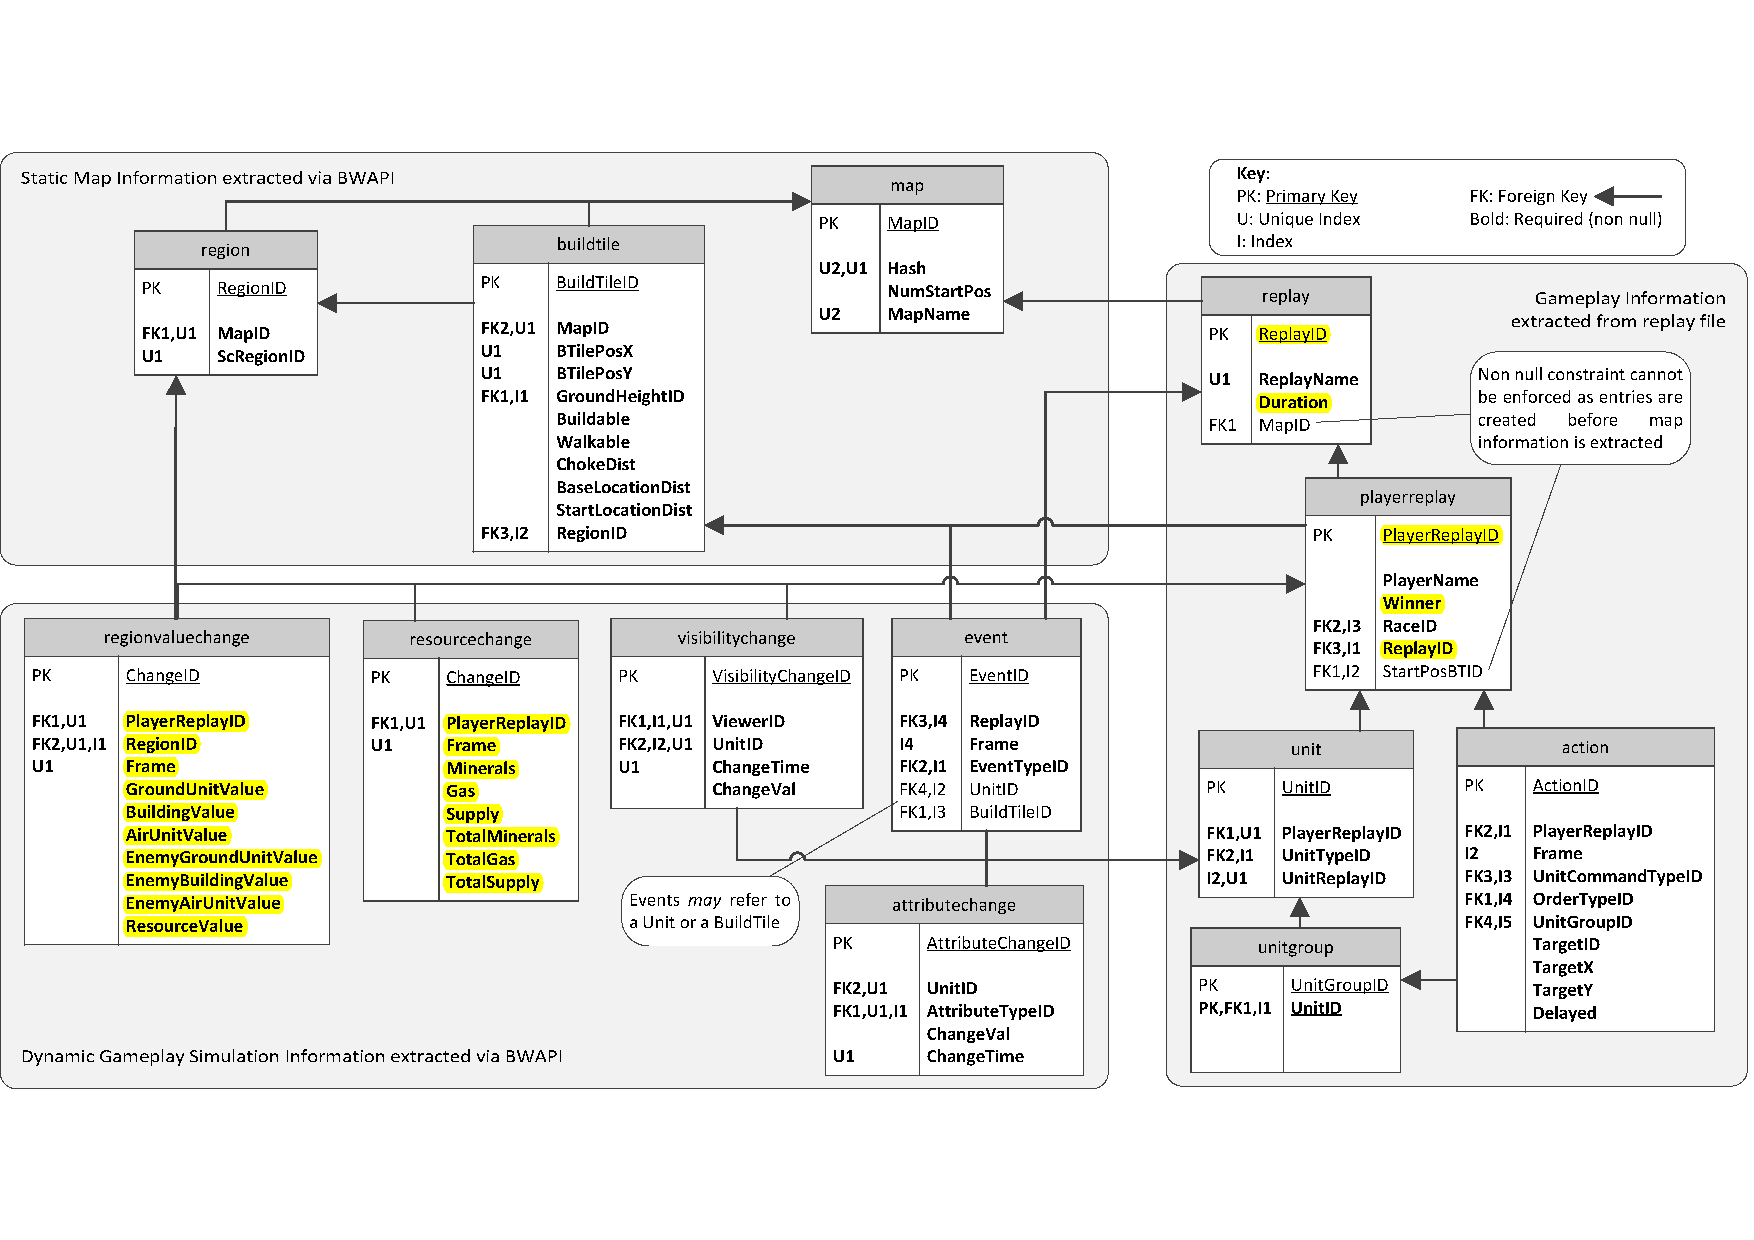
\includegraphics[scale=0.5]{figure/Robertson14DatabaseDiagramSeleccion.pdf}
  \caption{Selected features in databases. Original diagram by~\cite{DBLP:conf/flairs/RobertsonW14}}
  \label{fig:databaseSelection}
\end{figure*}

We present here the list of selected features, also exposed in
Figure~\ref{fig:databaseSelection}. Some of them are used only to organise the
data, the identifiers of replay, player and region.

\begin{itemize}
  \item replay: This table contais data about each match.
  \begin{itemize}
    \item ReplayID: Match identifier.
    %\item Duration: Duration of each match in frames, 15 frames per second.
  \end{itemize}
  \item playerreplay: This table contains data about a player in a match.
  \begin{itemize}
    \item PlayerReplayID: Player identifier.
    \item ReplayID: Match identifier.
    \item Winner: Winner of the match.
  \end{itemize}
  \item resourcechange: This table contains data associated to changes in player's resources.
  \begin{itemize}
    \item PlayerReplayID: Player identifier.
    \item Frame: Frame when the resource changes.
    \item Minerals: Amount of minerals of a player.
    \item Gas: Amount of gas of a player.
    \item Supply: Carrying capacity of a player.
    \item TotalMinerals: Total amount of minerals of a player, without costs.
    \item TotalGas: Total amount of minerals of a player, without costs.
    \item TotalSupply: Total amount of minerals of a player, without costs.
  \end{itemize}
  \item regionvaluechange: This table contains data associated to changes of a
  player in a map region. Each \emph{value} is the sum of the price of an unit,
  expressed as minerals and gas.
  \begin{itemize}
    \item PlayerReplayID: Player identifier.
    \item RegionID: Region of the map identifier.
    \item Frame: Frame when the value changes.
    \item GroundUnitValue: Value of ground units in this region.
    \item BuildingValue: Value of buildings in this region.
    \item AirUnitValue: Value of air units in this region.
    \item EnemyGroundUnitValue: Value of enemy ground units in this region.
    This value is estimated, the player knows the units they see of the enemy.
    \item EnemyBuildingValue: Value of enemy buildings in this region.
    This value is estimated, the player knows the units they see of the enemy.
    \item EnemyAirUnitValue: Value of enemy air units in this region.
    This value is estimated, the player knows the units they see of the enemy.
    \item ResourceValue: Value of resources in this region. This value is
    estimated, the player knows the units they see of the map.
    If the player doesn't know a region, they estimate this value as the maximum
    available in the region.
  \end{itemize}
\end{itemize}

The features related to a player are presented twice, one for each player.
Furthermore, a \emph{race} feature is used, as the races implied in the match.
As a consecuence, we have 28 features used in the modelling stage of the work.

\subsection{Data preprocessing}
\label{subsec:preprocess}

As we said in~\ref{subsec:selection}, each observation of the data has 28
features related to the resources and units of each player. We have to note
some little tips about the data organisation.

\begin{itemize}
  \item Values of \emph{Frame} are the instants when a whatever player has
  a minerals, gas or supply change. We did this election because in this games
  the basic resources are always changing due to necessity of them to buy
  units or buildings. This implies some missing values in the resources of
  the player who doesn't make a change in that frame, so we had to recover the
  last value of that resource to keep consistency.
  \item Values of \emph{value} of units and buildings doesn't occur in the
  same instant that the resources' changes. For this reason, as we did with
  \emph{Frame}, we had to recover the last value of the region values of
  each player, too.
  \item \emph{Value} depends of the region of the map. It's important in our
  approach to get a full \emph{value} measure, a value that represents all
  the player units or buildings, so we had to sum the \emph{value} of every
  region of the map.
\end{itemize}


\subsection{Exploratory Data Analysis}
\label{subsec:eda}

\section{\uppercase{Results}}
\label{sec:results}

\section{\uppercase{Conclusions}}
\label{sec:conclusions}

\section*{\uppercase{Acknowledgements}}
\label{sec:acknowledgements}

\vfill
\bibliographystyle{apalike}
{\small
\bibliography{prediction}}

\vfill
\end{document}
